
\documentclass[a4paper,20pt,dvipsnames, usenames]{extbook}

\usepackage{background}
\usepackage{xcolor}
\usepackage{graphicx}
\usepackage{hyperref}
\hypersetup{
	colorlinks,
	filecolor=[HTML]{054a40},
	linkcolor=[HTML]{054a40}
}
\usepackage{fancyhdr}
\addtolength{\headheight}{1.5cm} % make more space for the header
\pagestyle{fancyplain} % use fancy for all pages except chapter start
\lhead{
\includegraphics[height=2cm]{logo}} % left logo
%\rhead{
\includegraphics[height=2cm]{logo}} % right logo
%\renewcommand{\headrulewidth}{0pt} % remove rule below header
\usepackage{xepersian}
\settextfont{IRLotus}
\setlatintextfont{Times New Roman}
%\setdigitfont[Scale=1.1]{IRLotus}
\linespread{1.5}

\font\authorfont=IRTitr at 20pt
\author{\authorfont{دانشگاه فردوسی مشهد}}
\font\titlefont=IRTitr at 50pt
%
\font\subtitlefont=IRTitr at 25pt
\title{\titlefont{\textcolor[HTML]{04485f}{پهبار}}\\
		\subtitlefont{\textcolor[HTML]{04485f}{راهنمای استفاده از نرم‌افزار پیش‌بینی هوشمند بار}}}
\begin{document}
	\pagecolor[HTML]{f2f8e9}
	\backgroundsetup{contents= 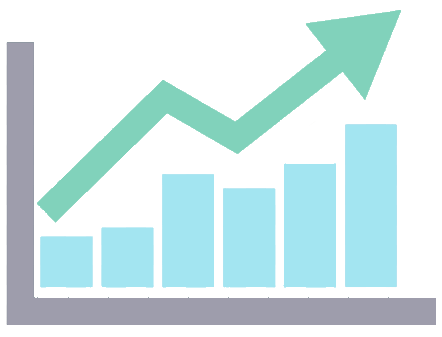
\includegraphics{icon.png}, opacity=0.08, scale = 1, angle = 0}
	\begin{titlepage}
		\centering
		
\includegraphics[width=0.15\textwidth]{logo}\par\vspace{2cm}
		{\scshape\titlefont{\textcolor[HTML]{04485f}{پهبار}}\\
			\subtitlefont{\textcolor[HTML]{04485f}{راهنمای استفاده از نرم‌افزار پیش‌بینی هوشمند بار}} \par}
		\vspace{1cm}
		{\scshape\Large \authorfont{دانشگاه فردوسی مشهد}\par}
		\vspace{1.5cm}
%		{\scshape1 بهمن 1399\par}
		
		\vfill
	\end{titlepage}
%	\maketitle
	\tableofcontents
	\chapter{معرفی پهبار}
	نرم‌افزار پیش‌بینی هوشمند بار (پهبار)، توسط جمعی از دانشجویان و فارغ‌التحصیلان دانشگاه فردوسی مشهد، به منظور پیش‌بینی کوتاه‌مدت مصرف برق، توسعه یافته است. این نرم‌افزار با استفاده از تکنیک یادگیری ماشین، قابلیت پیش‌بینی بار تا 10 روز آینده را دارد. پهبار با داده‌های بار از سال 1396 آموزش دیده است و هرچه داده‌ها افزایش پیدا کند و دوباره نرم‌افزار با داده‌های جدید آموزش داده شود، دقت آن در پیش‌بینی بالاتر خواهد رفت. 
	
	متغیرهای تأثیرگذار بر بار هر روز،‌اطلاعات تقویمی آن روز، اطلاعات تقویمی دو روز قبل (روز قبل از روزی که در آن پیش‌بینی انجام می‌شود) و هفته قبل، طول روز فردا، دو روز قبل و هفته قبل،‌اطلاعات آب و هوا، اطلاعات بار دو روز قبل و هفته قبل هستند. کافی است یک فایل
	\lr{Excel}
	شامل اطلاعات بار روز قبل از پیش‌بینی در نرم‌افزار بارگذاری شود، سایر اطلاعات مورد نیاز به طور اتوماتیک توسط نرم‌افزار دریافت شده و از آن‌ها برای پیش‌بینی بار روز بعد استفاده خواهد شد.
	
	در حال حاضر،‌ پهبار از وب‌سایت \lr{www.wunderground.com}، اطلاعات آب و هوا را دریافت می‌کند. به دلیل این که این وب‌سایت، پیش‌بینی آب و هوا را تنها تا 10 روز آینده در اختیار کاربران قرار می‌دهد، پهبار قادر به پیش‌بینی تا 10 روز آینده است.
	
\chapter{داده‌های ذخیره شده در نرم‌افزار}
با وارد کردن داده‌های روزانه بار،‌نرم‌افزار در طی فرآیند به‌روزرسانی، پس از گرفتن اطلاعات تقویمی و آب و هوایی مربوط به آن روز،‌ تمامی اطلاعات را ذخیره می‌کند. بنابراین، پس از بستن نرم‌افزار و اجرای دوباره آن، این اطلاعات هم‌چنان در نرم‌افزار هستند. 

\section{مشاهده تاریخ آخرین اطلاعات وارد شده}
آخرین روزی که اطلاعات آن وارد نرم‌افزار شده است در زبانه
\lr{Data}
در یک کادر کوچک در سمت چپ نشان داده می‌شود (شکل 
\ref{fig0}).
در این کادر، هم‌چنین، آخرین تاریخی که آموزش مدل انجام شده نشان داده شده است. با انتخاب دیتاست مورد نظر (با نیروگاه یا بدون نیروگاه)، (شکل
\ref{fig0-1}
) آخرین تاریخ وارد شده در همان دیتاست و آخرین تاریخی که نرم‌افزار با آن دیتاست آموزش دیده است نشان داده خواهد شد. 
\begin{figure}[!h]
	\centering
	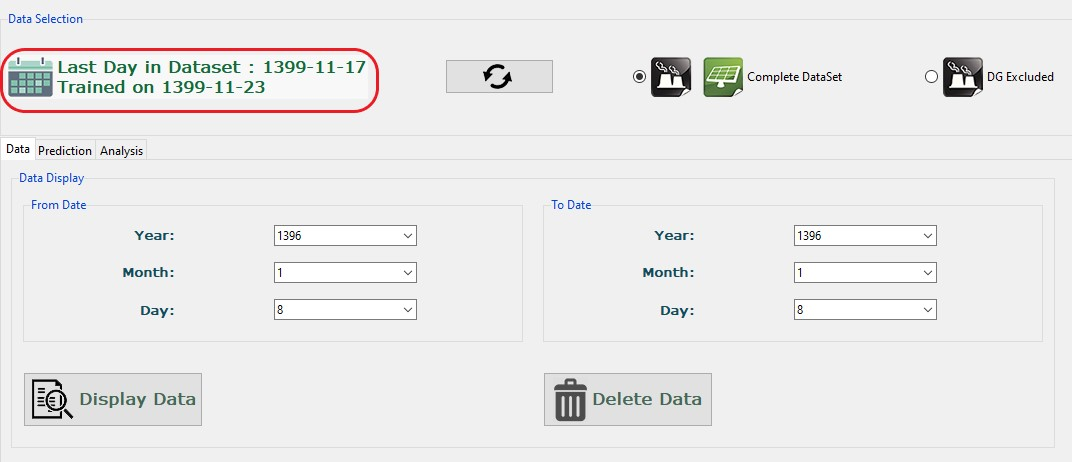
\includegraphics[width = \textwidth]{fig0}
	\caption{مشاهده تاریخ آخرین اطلاعات وارد شده و تاریخ آخرین آموزش نرم‌افزار}
	\label{fig0}
\end{figure}
\begin{figure}[!h]
	\centering
	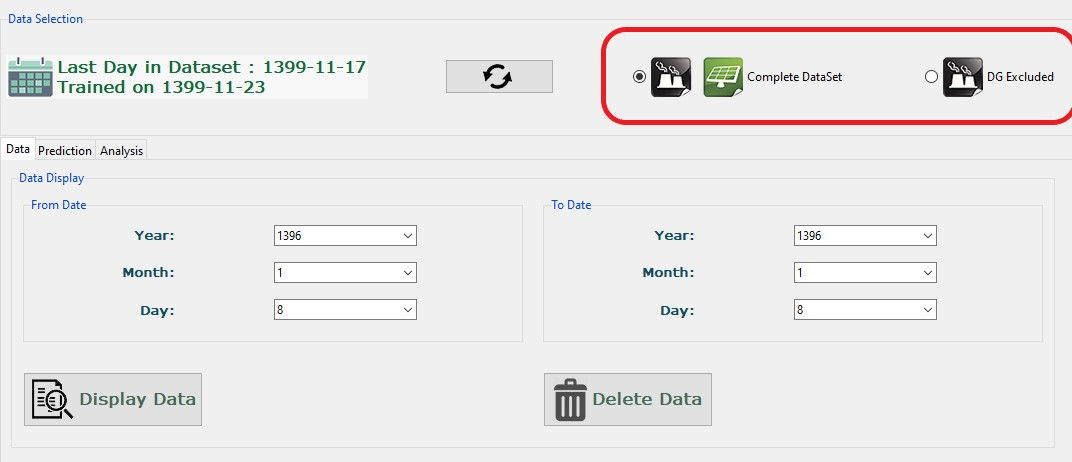
\includegraphics[width = \textwidth]{fig1}
	\caption{انتخاب دیتاست}
	\label{fig0-1}
\end{figure}

گزینه
\lr{Complete Dataset}
مربوط به دیتاست "با نیروگاه" و گزینه 
\lr{DG Excluded}
مربوط به دیتاست "بدون نیروگاه" است.
با کلیک بر روی دکمه سمت راست کادر در هر زمان، تاریخ‌های نشان داده شده در این کادر، ‌به‌روز‌رسانی می‌شوند.



\section{نمایش داده‌ها}

می‌توان در زبانه \lr{Data} پس از انتخاب بازه مورد نظر،‌اطلاعات موجود در نرم‌افزار مربوط به آن بازه را مشاهده کرد. 
مراحل مشاهده داده‌ها به شرح زیر است.
\begin{itemize}
	\item
	انتخاب دیتاست مورد نظر (شکل \ref{fig0-1})
	
	\item
	انتخاب بازه زمانی و کلیک بر روی گزینه 
	\lr{Display Data}
(شکل
\ref{fig2}).
	\begin{figure}[!h]
		\centering
		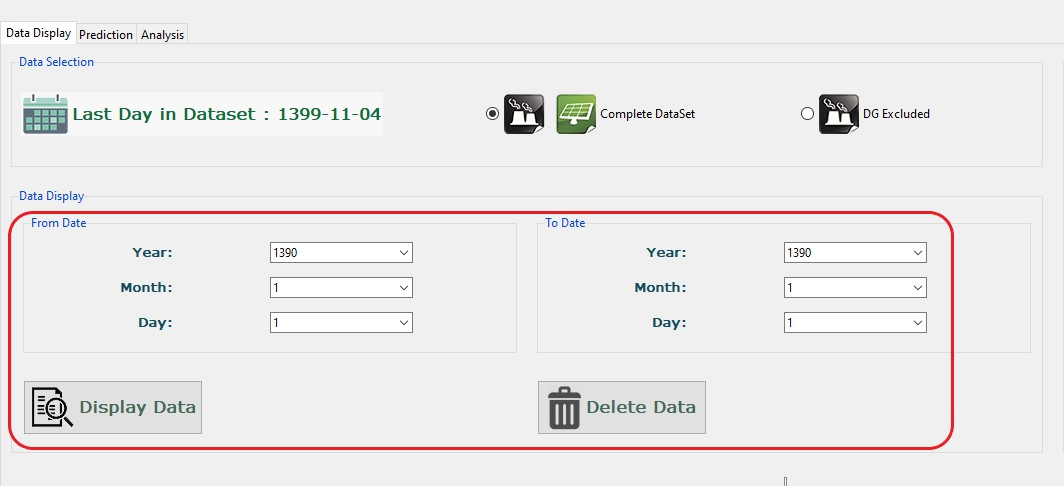
\includegraphics[width = \textwidth]{fig16}
		\caption{انتخاب بازه زمانی}
		\label{fig2}
	\end{figure}
	اگر تاریخ وارد شده در دیتاست موجود نباشد،‌‌ پیغام خطا دریافت خواهید نمود.
	\item
	در صورتی که بازه انتخاب شده در دیتاست موجود باشد، با کلیک بر روی گزینه 
	\lr{Display Data}
	اطلاعات موجود در نرم‌افزار در پایین صفحه به نمایش درمی‌آیند (شکل
	\ref{fig4}). ویژگی‌های نشان داده شده، عمده ویژگی‌هایی است که نرم‌افزار برای پیش‌بینی از آن‌ها استفاده می‌کند.
	\begin{figure}[!h]
		\centering
		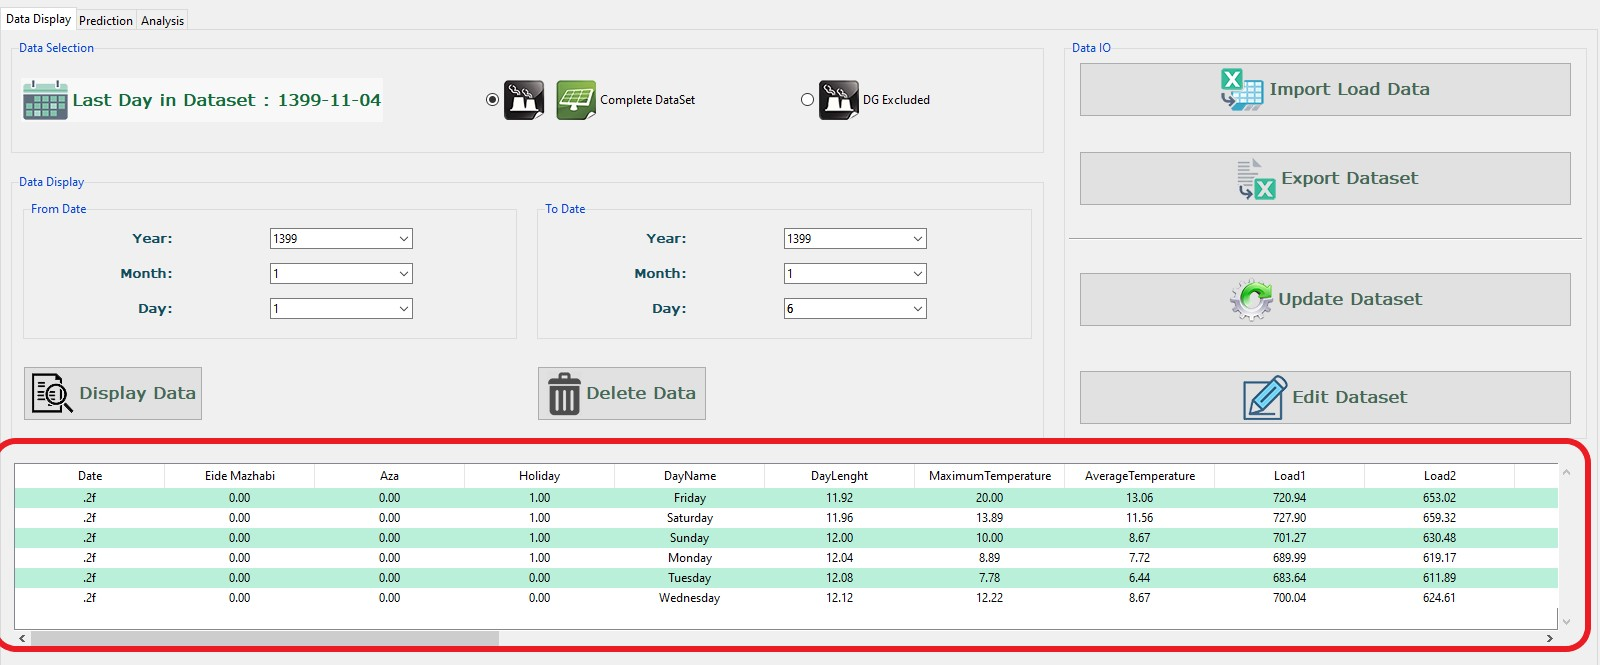
\includegraphics[width = \textwidth]{fig17}
		\caption{نمایش داده‌ها}
		\label{fig4}
	\end{figure}
\end{itemize}

\section{حذف داده‌های روزهای مشخص}
گاهی ممکن است داده‌های مربوط به بار یک روز مشخص وارد نرم‌افزار شده باشد و بعد از مدتی متوجه شوید که داده وارد شده مشکلی داشته است و داده درست نیز در دسترس نیست. در این صورت، بهترین راه حذف کردن داده آن روز است. در این حالت،‌نرم‌افزار به صورت اتوماتیک، داده حذف شده را با مقادیر پیش‌بینی شده مربوط به آن روز جایگزین می‌کند. مراحل حذف داده‌های یک بازه مشخص به صورت زیر است:
\begin{itemize}
	\item
	دیتاست مورد نظر را انتخاب کنید (شکل	
	\ref{fig5-1}).
	\begin{figure}[!h]
		\centering
		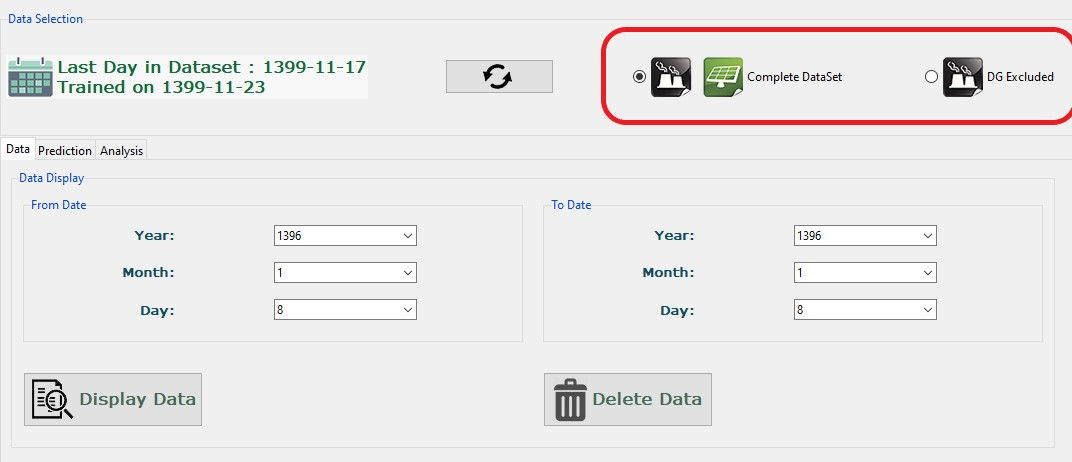
\includegraphics[width = \textwidth]{fig1}
		\caption{انتخاب دیتاست}
		\label{fig5-1}
	\end{figure}
	\item
	پس از انتخاب بازه مورد نظر، بر روی گزینه 
	\lr{Delete Data}
	کلیک کنید (شکل
	\ref{fig28}).
	
	\begin{figure}[!h]
		\centering
		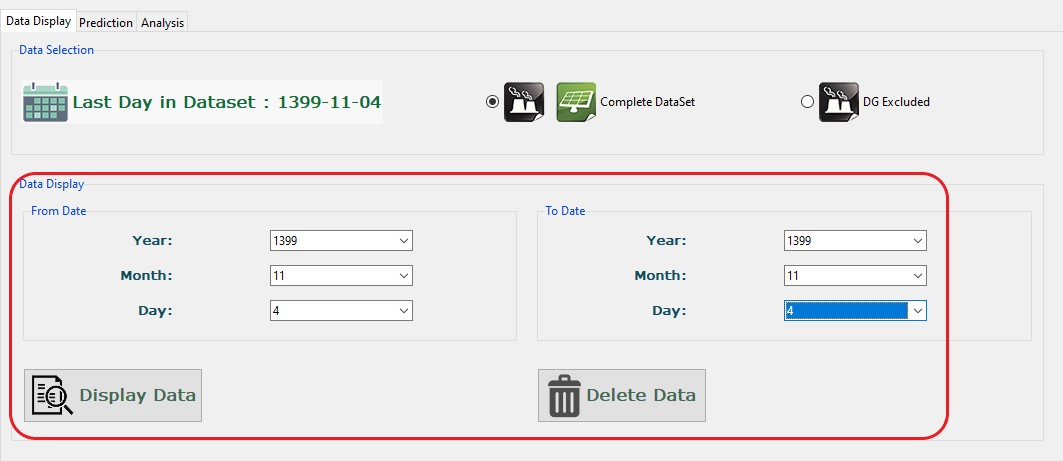
\includegraphics[width = \textwidth]{fig26}
		\caption{انتخاب بازه و حذف دیتا}
		\label{fig28}
	\end{figure}

\item
پیغام زیر نمایش داده خواهد شد (شکل
\ref{fig29}).
در صورت اطمینان از حذف داده‌ها بر روی گزینه
\lr{Yes}
کلیک کنید.
\begin{figure}[!h]
	\centering
	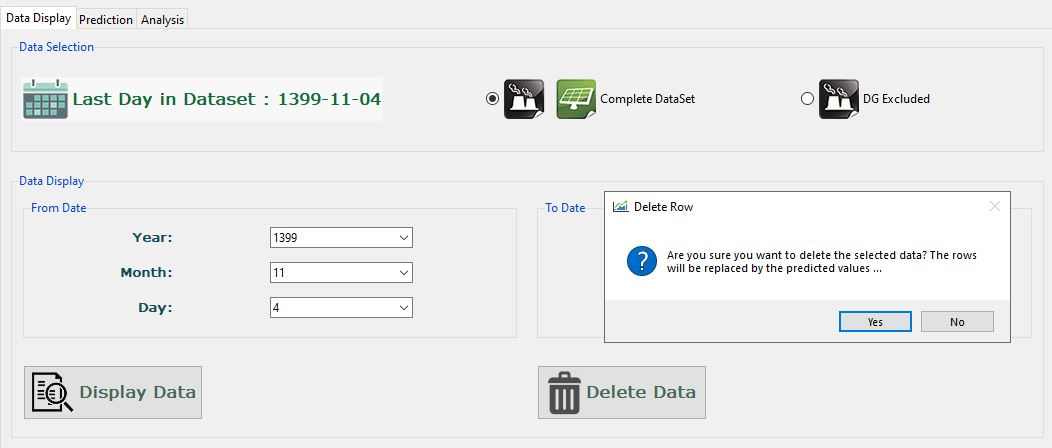
\includegraphics[width = \textwidth]{fig27}
	\caption{پیغام اطمینان از حذف داده‌ها}
	\label{fig29}
\end{figure}
\item
\textcolor{red}{در این مرحله لازم است به اینترنت دسترسی داشته باشید.}
منتظر بمانید تا بار مربوط به بازه انتخاب شده، پیش‌بینی و مقادیر قبلی با مقادیر پیش‌بینی شده جایگزین شوند. در این صورت پیغام زیر نمایش داده خواهد شد (شکل
\ref{fig30}).

\begin{figure}[!h]
	\centering
	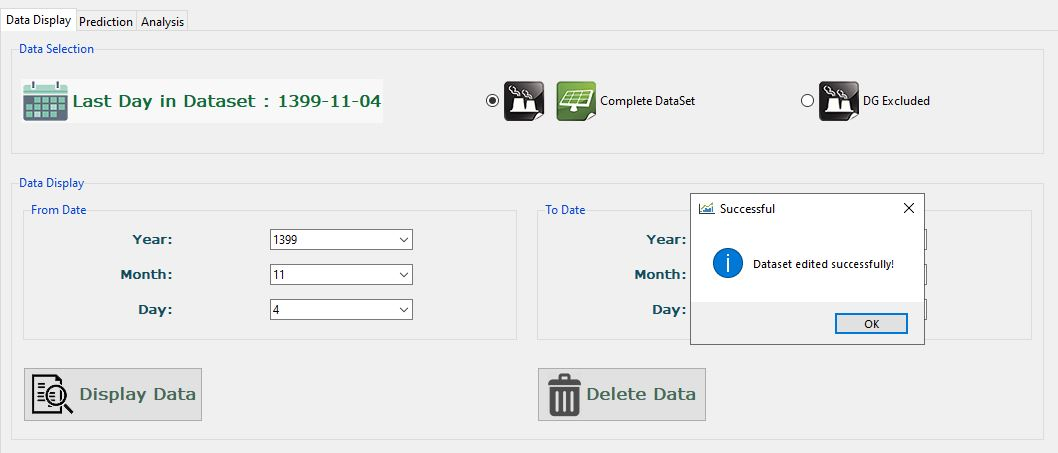
\includegraphics[width = \textwidth]{fig28}
	\caption{پیغام حذف و جایگزینی موفقیت‌‌آمیز داده‌ها}
	\label{fig30}
\end{figure}

\end{itemize}
\section{استخراج داده‌ها}	
در پهبار، گزینه‌ای برای استخراج داده‌های ذخیره شده در نرم‌افزار تعبیه شده است. بدین منظور ابتدا نوع دیتاست (با نیروگاه یا بدون نیروگاه) را انتخاب کنید (شکل
\ref{fig5}).
\begin{figure}[!h]
	\centering
	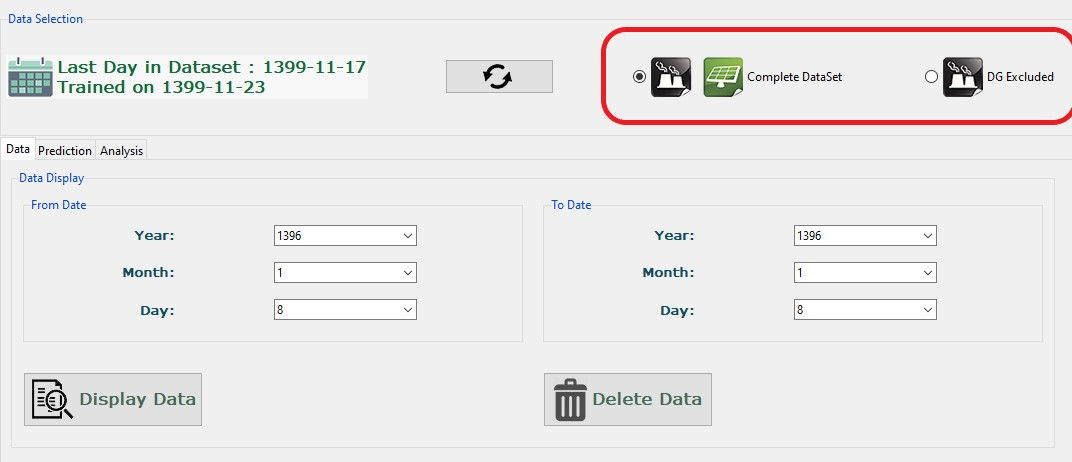
\includegraphics[width = \textwidth]{fig1}
	\caption{انتخاب دیتاست}
	\label{fig5}
\end{figure}
سپس بر روی گزینه
\LR{Export Dataset}
کلیک نمایید و با انتخاب محل مورد نظر،‌کلیه اطلاعات مربوط به آن دیتاست را ذخیره کنید (شکل
\ref{fig6}).
\begin{figure}[!h]
	\centering
	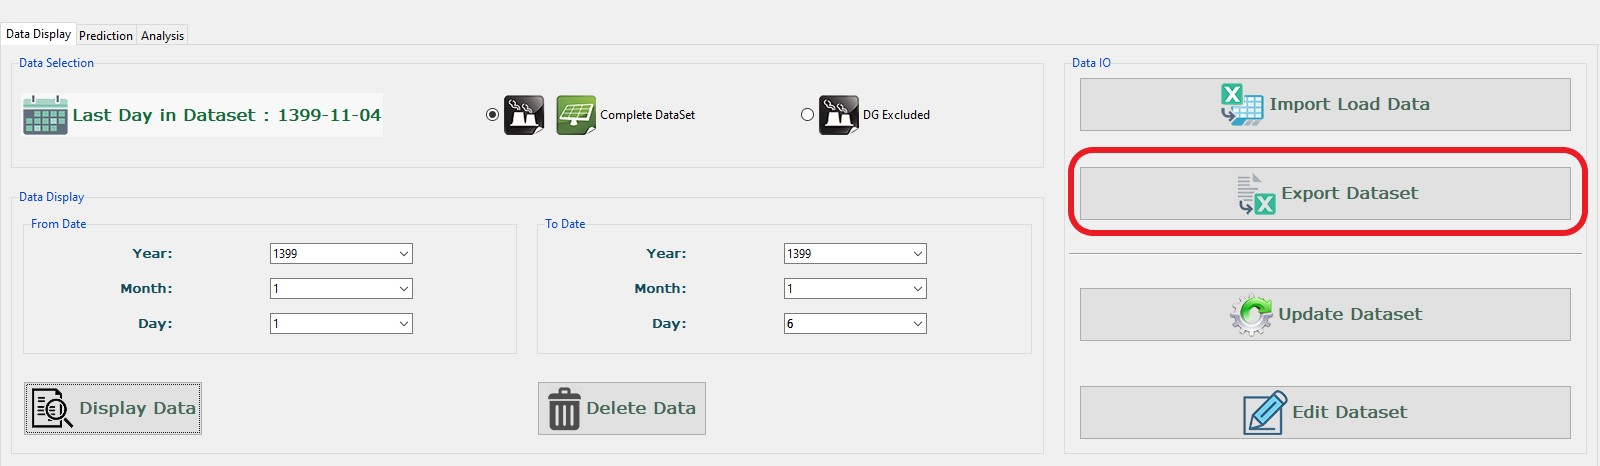
\includegraphics[width = \textwidth]{fig19}
	\caption{استخراج دیتاست}
	\label{fig6}
\end{figure}
در صورت موفقیت‌آمیز بودن استخراج داده‌ها،‌پیغام زیر را دریافت خواهید نمود (شکل
\ref{fig7}).
\begin{figure}[!h]
	\centering
	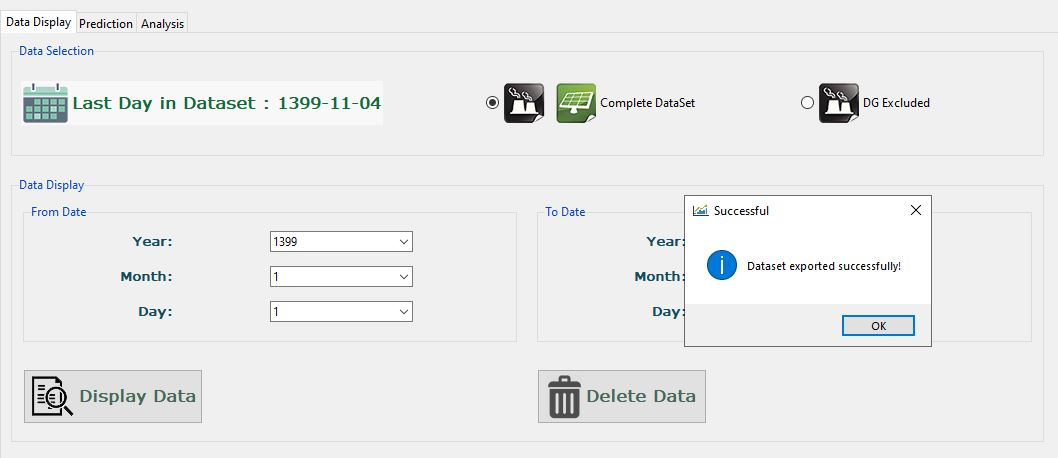
\includegraphics[width = \textwidth]{fig20}
	\caption{پیغام استخراج موفق داده‌ها}
	\label{fig7}
\end{figure}

\section{تکمیل (به روز رسانی) داده‌ها}
\underline{\textcolor{red}{توجه:
		از اتصال اینترنت اطمینان حاصل کنید!}}

بهتر است قبل از انجام پیش‌بینی، دیتاست‌ها کامل شده باشند. در صورتی که داده‌ها تا روز قبل در نرم‌افزار قرار داده نشود، بار تمامی روزهایی که در اطلاعات موجود نیست، تا روزی که می‌خواهیم بار آن را پیش‌بینی کنیم، پیش‌بینی می‌شود. این امر باعث افزایش خطای پیش‌بینی خواهد شد. پس ابتدا دیتاست مورد نظر را انتخاب کرده (شکل
\ref{fig31}
) و در کادر سمت چپ، آخرین تاریخی که داده موجود است را بررسی کنید. اگر داده‌ای پس از آخرین روزی که نمایش داده شده دارید، طبق مراحل زیر، دیتاست مورد نظر را آپدیت کنید:

\begin{figure}[!h]
	\centering
	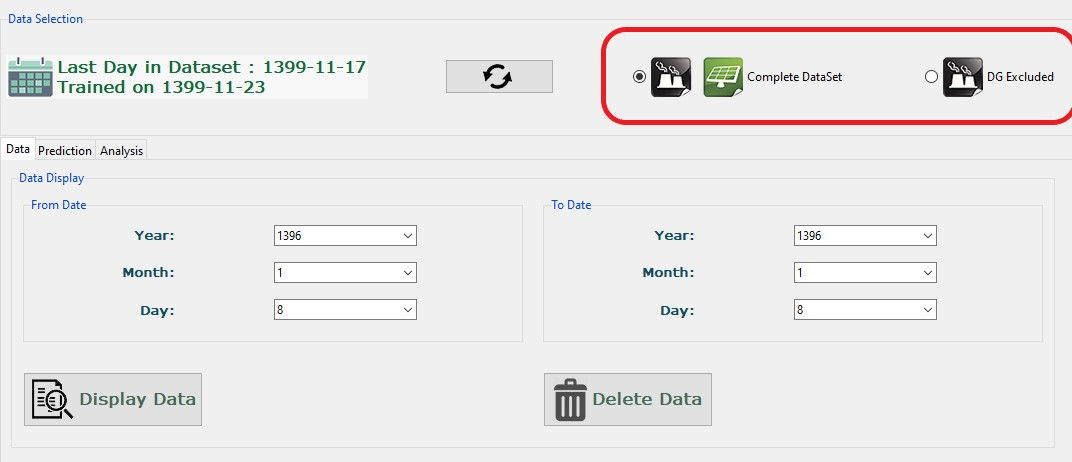
\includegraphics[width = \textwidth]{fig1}
	\caption{انتخاب دیتاست}
	\label{fig31}
\end{figure}

ابتدا فایل حاوی بار روزهایی که در نرم‌افزار موجود نیست را بارگذاری کنید. این فایل باید در فرمت اکسل و  دارای یک ستون به نام "تاریخ" و ستون‌های ساعات به شکل 
\lr{H1}
تا
\lr{H24}
باشد. تاریخ‌ها باید در فرمت "روز/ماه/سال" (به طور مثال، 1399/11/17) در ستون "تاریخ" آمده باشند. برای وارد کردن این فایل، مراحل زیر را دنبال کنید.

روی گزینه
\lr{Import Load Data}
کلیک کنید (شکل
\ref{fig15}
).
\begin{figure}[h]
	\centering
	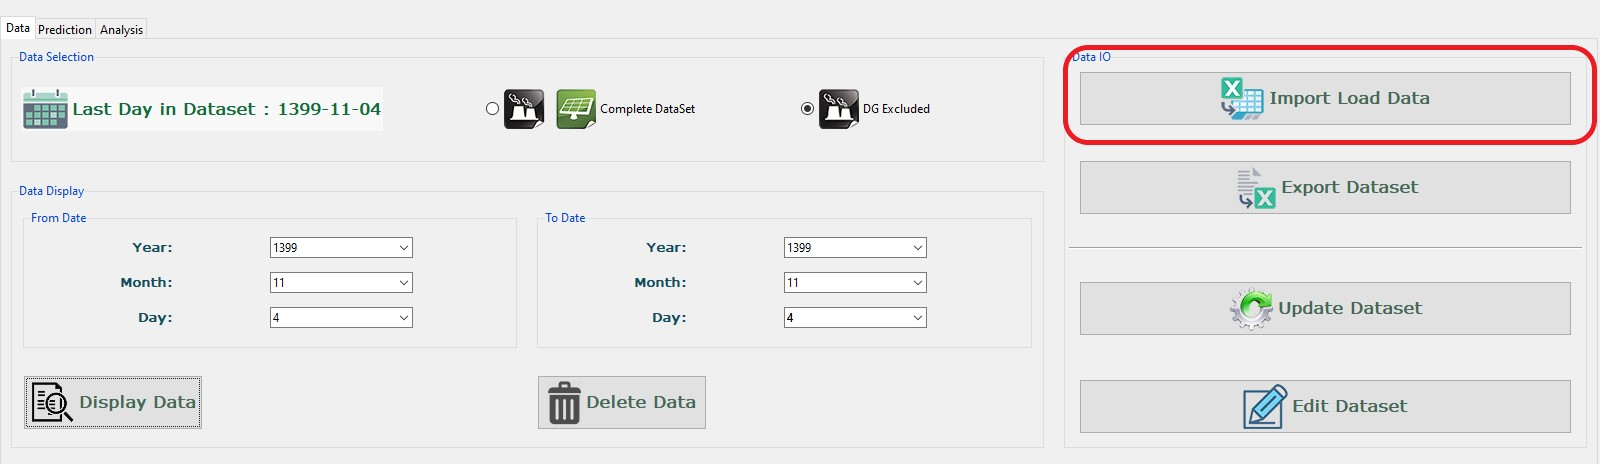
\includegraphics[width = \textwidth]{fig2}
	\caption{وارد کردن اطلاعات بار}
	\label{fig15}
\end{figure}
فایل مورد نظر را انتخاب کرده و بر روی گزینه
\lr{Open}
کلیک کنید.
در صورت دریافت پیام زیر، نرم‌افزار، فایل اطلاعات بار را با موفقیت دریافت کرده است (شکل
\ref{fig17}).
\begin{figure}[h]
	\centering
	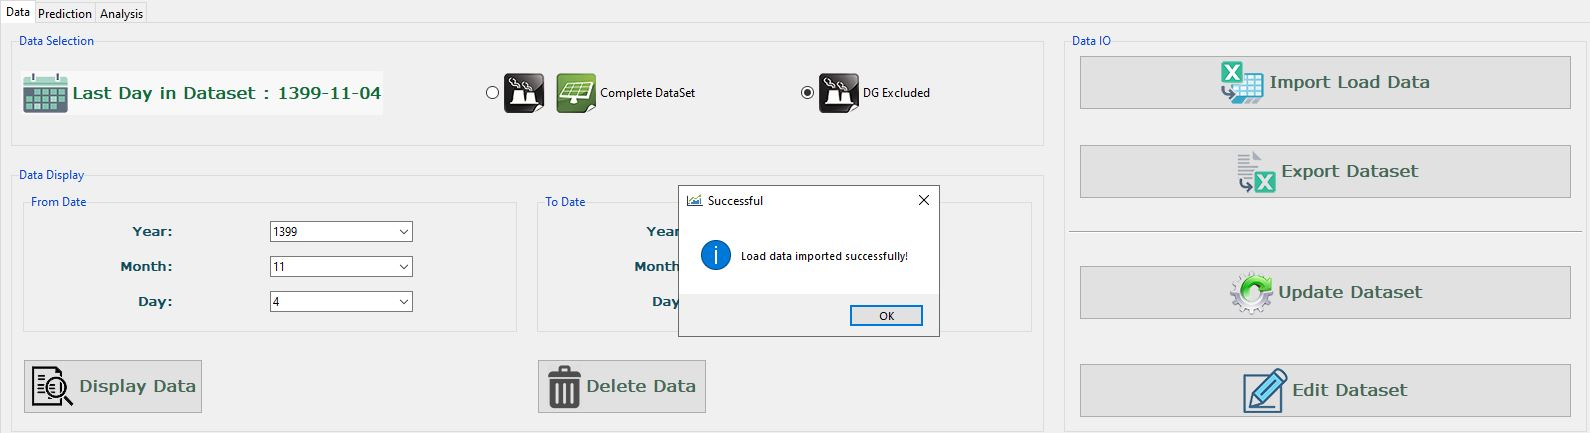
\includegraphics[width = \textwidth]{fig4}
	\caption{پیغام دریافت موفقیت‌آمیز اطلاعات بار}
	\label{fig17}
\end{figure}

حالا می‌توان با استفاده از اطلاعات وارد شده و با اتصال به اینترنت، دیتاست را تکمیل کرد. با کلیک روی گزینه
\lr{Update Dataset}
نرم‌افزار به صورت خودکار اطلاعات مورد نیاز خود از جمله اطلاعات بار،‌آب و هوا و اطلاعات تقویمی را تا آخرین روزی که در فایل بارگذاری شده وجود دارد به‌روزرسانی می‌کند (شکل
\ref{fig18}).
\begin{figure}[!h]
	\centering
	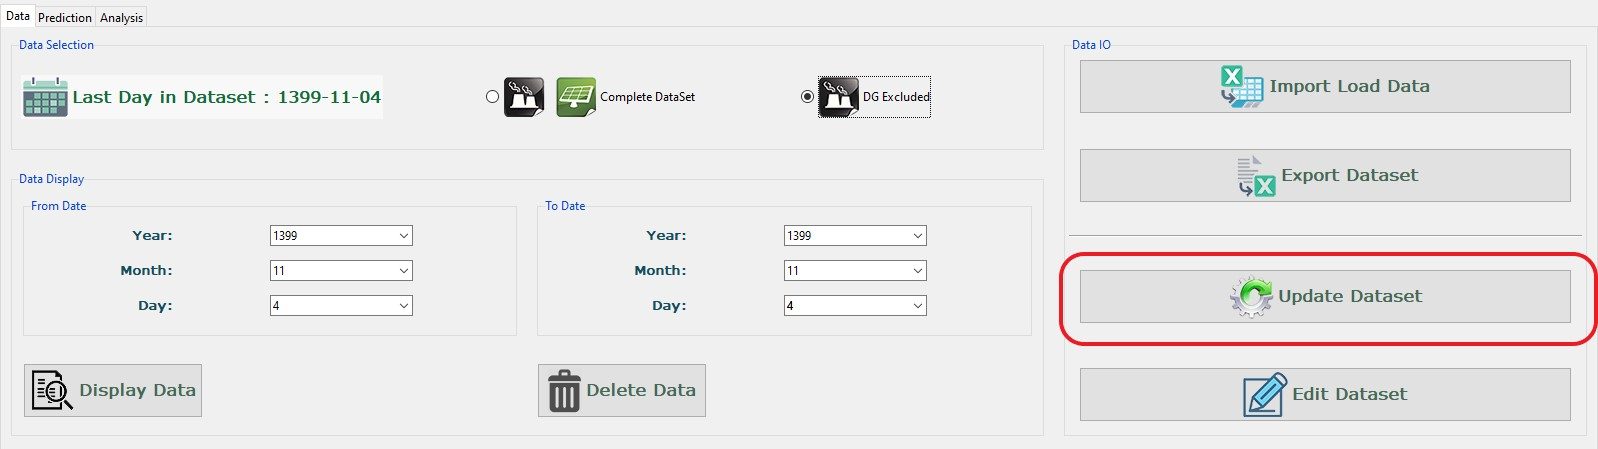
\includegraphics[width = \textwidth]{fig5}
	\caption{تکمیل (به‌روزرسانی) اطلاعات}
	\label{fig18}
\end{figure}

چند دقیقه صبر کنید تا اطلاعات به‌روزرسانی شود.

اگر اتصال به اینترنت برقرار نباشد یا در اطلاعات بار مشکلی وجود داشته باشد، پیغام خطا دریافت خواهید کرد.

\textcolor{red}{\textbf{توجه:}در این صورت، ترجیحاً پیش‌بینی نباید انجام شود. زیرا به روز نبودن اطلاعات بر دقت پیش‌بینی اثر خواهد گذاشت.}

اگر اطلاعات بار به طور کامل به نرم‌افزار داده شده باشد و اتصال اینترنت برقرار باشد،‌ نرم‌افزار قادر به به‌روزرسانی اطلاعات است و پس از انجام به‌روزرسانی، پیام زیر به کاربر نمایش داده می‌شود (شکل
\ref{fig21}).
\begin{figure}[!h]
	\centering
	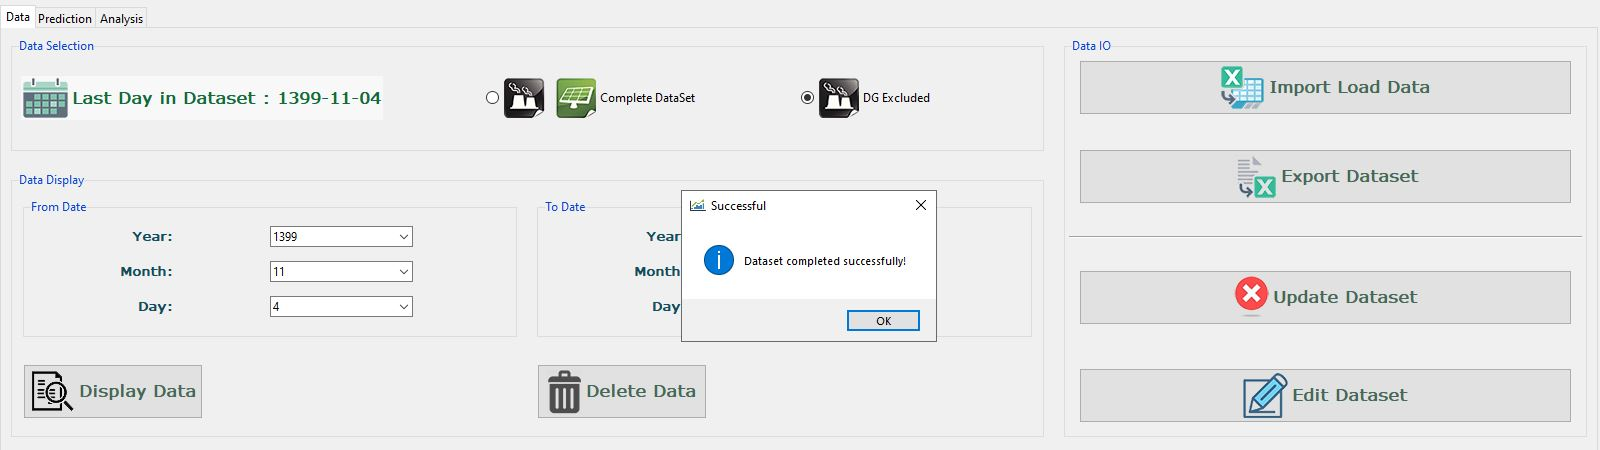
\includegraphics[width = \textwidth]{fig8}
	\caption{تکمیل موفقیت‌آمیز اطلاعات}
	\label{fig21}
\end{figure}

\section{تغییر داده‌های بار گذشته}
فرض کنید برای پیش‌بینی بار بدون نیروگاه روز 3 دی، اطلاعات بار بدون نیروگاه روز 1 دی را قبلاً وارد نموده‌ایم، در نرم‌افزار ذخیره شده و پیش‌بینی را انجام داده‌ایم. امروز در روز 3 دی متوجه شده‌ایم که در اطلاعات روز 1 دی خطایی وجود داشته و لازم است امروز آن را اصلاح کنیم. برای اصلاح داده‌های هر روز، ابتدا بار صحیح را در نرم‌افزار بارگذاری کنید. بار صحیح باید در قالب یک فایل اکسل با فرمت زیر باشد (شکل
\ref{fig8}).
\begin{figure}[!h]
	\centering
	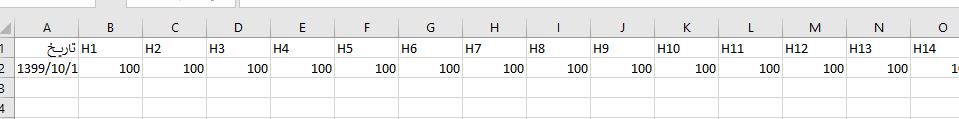
\includegraphics[width = \textwidth]{fig21}
	\caption{فرمت داده‌های بار}
	\label{fig8}
\end{figure}
فایل را از طریق گزینه
\lr{Import Load Data}
در نرم‌افزار بارگذاری کنید (شکل
\ref{fig9}).
\begin{figure}[!h]
	\centering
	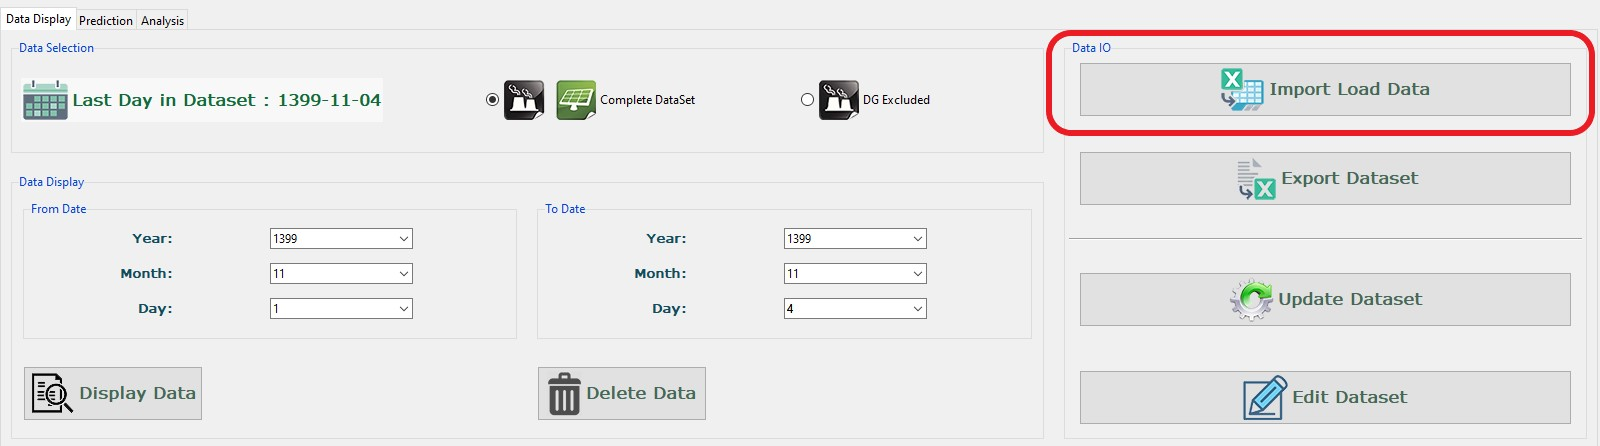
\includegraphics[width = \textwidth]{fig22}
	\caption{بارگذاری فایل اطلاعات صحیح بار}
	\label{fig9}
\end{figure}
سپس بر روی گزینه
\lr{Edit Dataset}
کلیک کنید. با کلیک بر روی این گزینه پیغام زیر ظاهر خواهد شد(شکل
\ref{fig10}). اگر اطمینان دارید که می‌خواهید داده‌های آن روز را تغییر دهید گزینه 
\lr{Yes}
را انتخاب نمایید.
\begin{figure}[!h]
	\centering
	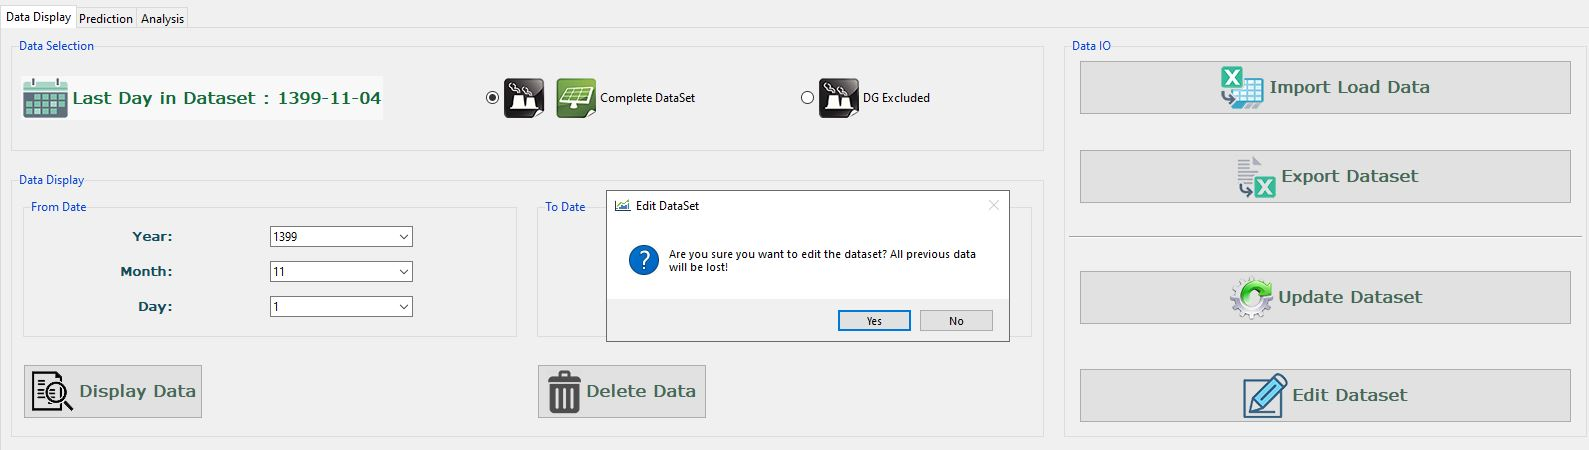
\includegraphics[width = \textwidth]{fig23}
	\caption{اطمینان از تغییر داده‌ها}
	\label{fig10}
\end{figure}
با کلیک بر روی گزینه 
\lr{Yes}
داده‌های روز 1 دی اصلاح خواهد شد. در این صورت پیغام زیر نمایش داده می‌شود (شکل
\ref{fig11}).
\begin{figure}[!h]
	\centering
	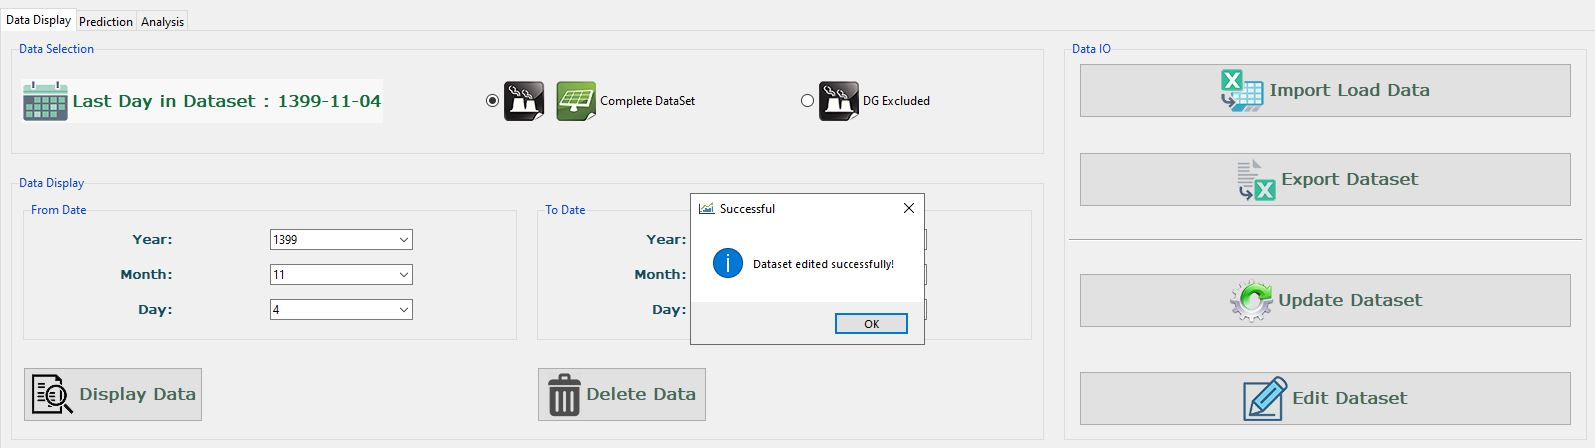
\includegraphics[width = \textwidth]{fig24}
	\caption{پیغام اصلاح موفقیت‌آمیز داده‌ها}
	\label{fig11}
\end{figure}
\chapter{آموزش نرم‌افزار}
پهبار،‌ براساس تکنیک یادگیری ماشین، به پیش‌بینی مصرف برق می‌پردازد. در واقع، با ذخیره اطلاعات بار در نرم‌افزار،‌ پهبار به طور اتوماتیک، سایر اطلاعاتی که برای پیش‌بینی نیاز دارد را از طریق وب‌سرویس‌های انتخاب شده استخراج می‌کند و وقتی به تمامی داده‌های مورد نیاز دست پیدا کرد، می‌تواند به وسیله آن‌ها برای پیش‌بینی بار آمادگی کسب کند. در واقع لازم است با این داده‌ها آموزش ببیند. بنابراین، اگر داده‌های جدید به نرم‌افزار وارد کنیم (به طور مثال پس از ورود یک هفته داده جدید)،‌ بهتر است پهبار با داده‌های جدید نیز آموزش داده شود تا بتواند با دقت بالاتری بار را پیش‌بینی کند. بنابراین 
\textbf{\underline{\textcolor{red}{حداقل یک روز در هفته،‌ نرم‌افزار را آموزش دهید}}.}

\textcolor{red}{توجه: اگر داده‌ای در دیتاست وجود دارد که از درستی آن اطمینان ندارید، یا در آینده قصد تغییر آن را دارید، از آموزش نرم‌افزار خودداری کنید. این امر ممکن است باعث بالا رفتن خطای پیش‌بینی شود.}
 

برای آموزش کافی است به زبانه 
\lr{Prediction}
بروید و نوع دیتاست را انتخاب کنید (با نیروگاه یا بدون نیروگاه) (شکل
\ref{fig12}).
\begin{figure}[!h]
	\centering
	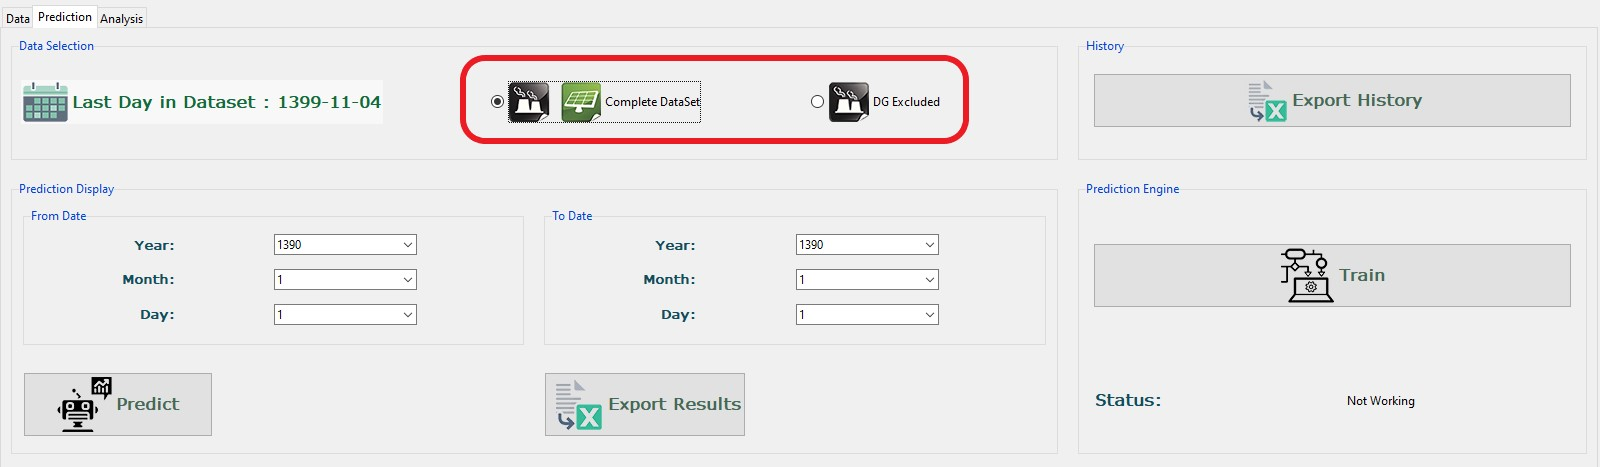
\includegraphics[width = \textwidth]{fig35}
	\caption{انتخاب دیتاست}
	\label{fig12}
\end{figure}

سپس بر روی گزینه 
\lr{Train}
کلیک کنید. روند آموزش نرم‌افزار شروع شده و گزینه
\lr{Train}
غیرفعال می‌شود (شکل
\ref{fig13}). 
\begin{figure}[!h]
	\centering
	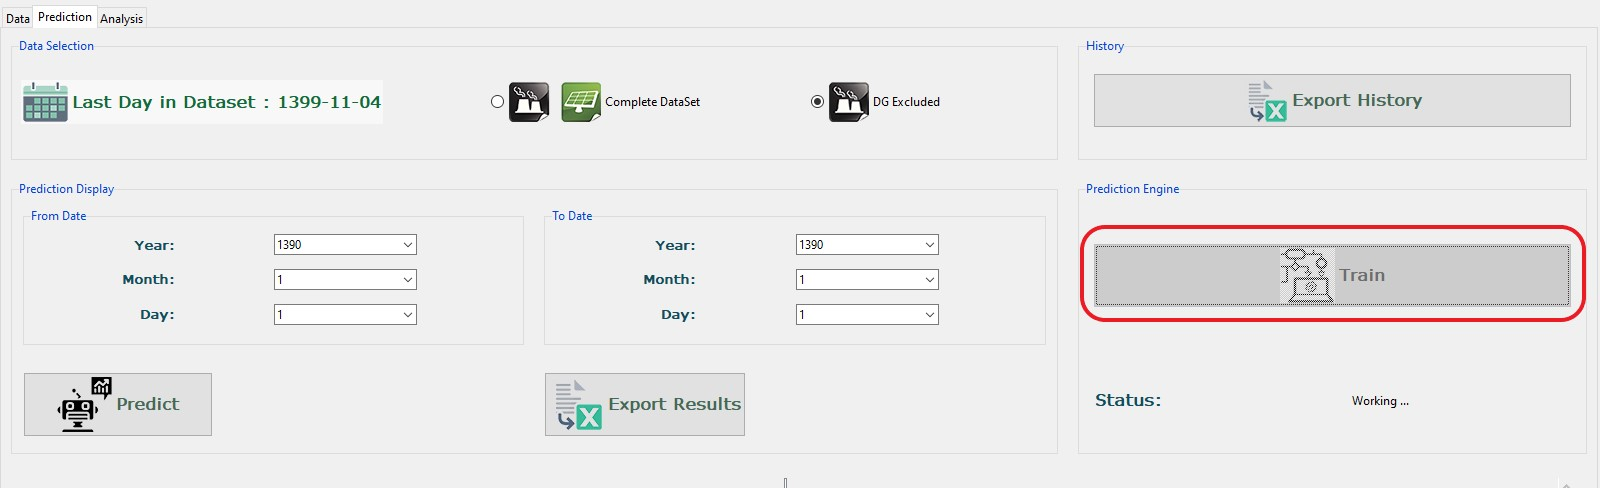
\includegraphics[width = \textwidth]{fig25}
	\caption{آموزش نرم‌افزار}
	\label{fig13}
\end{figure}
آموزش پهبار، حداکثر 3 الی 4 دقیقه زمان می‌برد. 

\underline{\textcolor{red}{لطفاً‌ در زمان آموزش، به هیچ عنوان نرم‌افزار را نبندید.}}

پس از اتمام آموزش، گزینه
\lr{Train}
دوباره فعال شده و می‌توانید با نرم‌افزار کار کنید یا آن را ببندید.

بهتر است در هر زمان که پهبار را آموزش می‌دهید، برای هر دو دیتاست این کار را انجام دهید. به این صورت که پس از آموزش با یک دیتاست، دیتاست دیگر را انتخاب کنید و مجدداً گزینه
\lr{Train}
را بزنید.
\chapter{پیش‌بینی}
در ابتدا، به زبانه 
\lr{Prediction}
رفته و نوع پیش‌بینی (با نیروگاه یا بدون نیروگاه) را انتخاب کنید (شکل
\ref{fig14}).
\begin{figure}[!h]
	\centering
	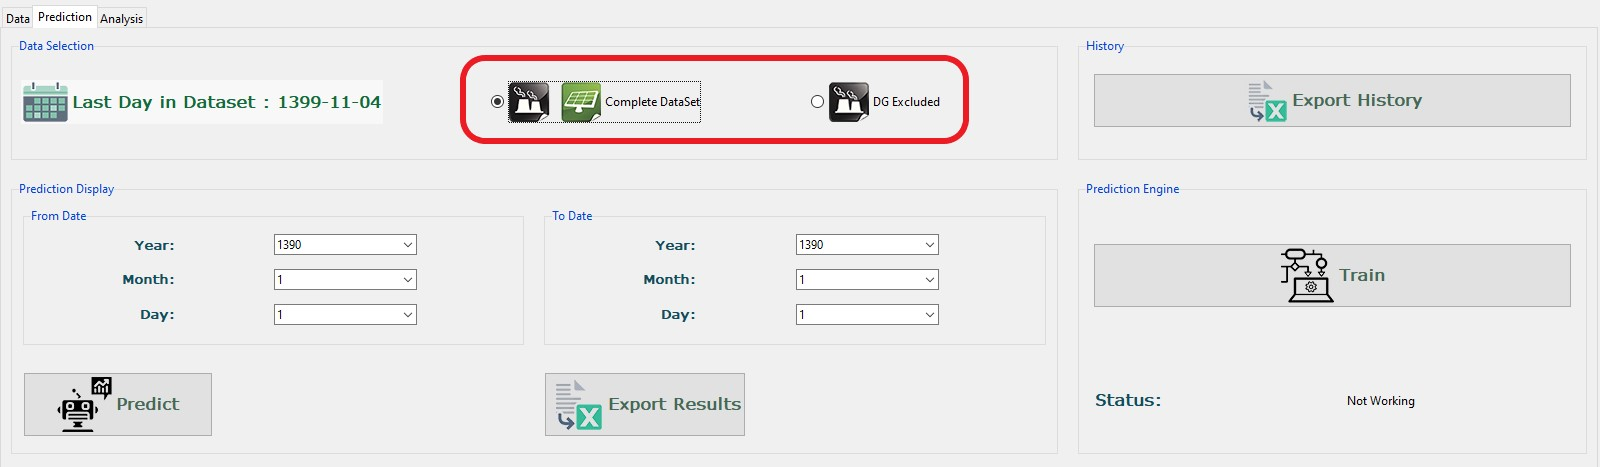
\includegraphics[width = \textwidth]{fig35}
	\caption{انتخاب دیتاست}
	\label{fig14}
\end{figure}
بهتر است در هنگام پیش‌بینی، دیتاست‌ها کامل باشند. یعنی اطلاعات تا روز قبل در دیتاست وارد شده باشد. وارد کردن و تکمیل اطلاعات در فصل اول توضیح داده شده است. در غیر این صورت، ممکن است خطای پیش‌بینی بالا برود.

پس از کامل کردن دیتاست، حتی اگر نرم‌افزار را ببندید و مجدداً باز کنید، چون نرم‌افزار تمامی اطلاعات مورد نیاز را دارد،‌ نیازی به بارگذاری مجدد فایل بار روز قبل نیست. 

در مرحله بعد، کافی است در بخش
\lr{Prediction Display}
بازه مورد نظر را انتخاب کرده و بر روی گزینه
\lr{Predict}
کلیک نمایید (شکل
\ref{fig24}). در این مرحله هم لازم است به اینترنت دسترسی داشته باشید.
 \begin{figure}[!h]
	\centering
	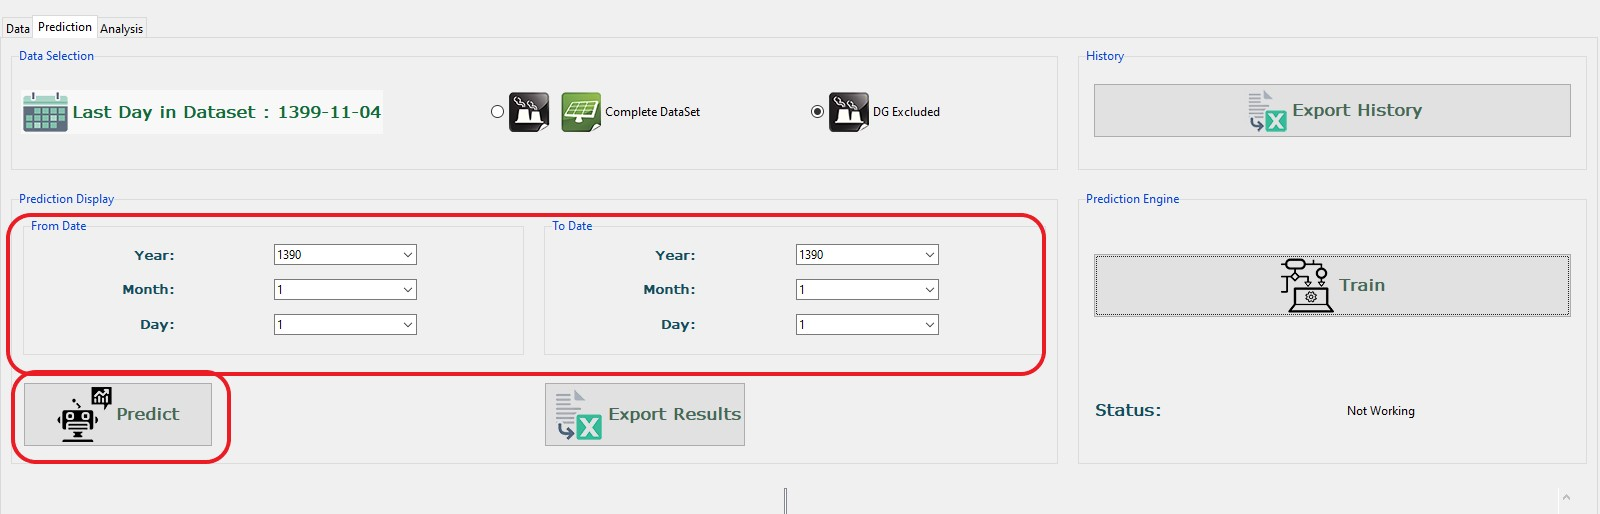
\includegraphics[width = \textwidth]{fig11}
	\caption{انتخاب بازه زمانی}
	\label{fig24}
\end{figure}
در صورت عدم اتصال به اینترنت یا وجود مشکلات دیگر نظیر عدم اطلاعات آموزش نرم‌افزار، پیش‌بینی انجام نشده و پیغام خطا نمایش داده می‌شود.

در صورت موفقیت‌آمیز بودن پیش‌بینی پیغام زیر به همراه اطلاعات پیش‌بینی شده نمایش داده می‌شود (شکل
\ref{fig26}).
\begin{figure}[!h]
	\centering
	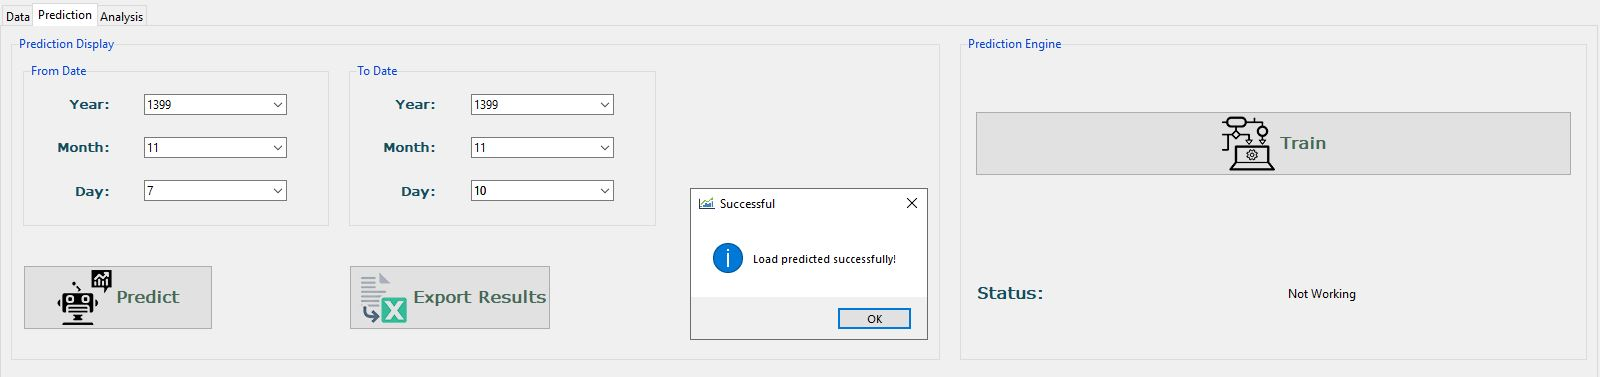
\includegraphics[width = \textwidth]{fig13}
	\caption{پیش‌بینی موفقیت‌آمیز}
	\label{fig26}
\end{figure}

برای استخراج بار پیش‌بینی شده در قالب فایل اکسل، بر روی گزینه
\lr{Export Prediction}
کلیک کنید و فایل را در محل مورد نظر ذخیره نمایید (شکل
\ref{fig27}).
\textcolor{red}{می‌توانید برای استخراج پیش‌بینی، تاریخ پیش‌بینی را تغییر دهید. در واقع، در هر زمان قابلیت دسترسی به پیش‌بینی‌های گذشته هم وجود دارد و اگر قبلاٌ بار روز مورد نظر پیش‌بینی شده باشد، بدون این که لازم باشد دوباره پیش‌بینی انجام شود، می‌توانید نتایج آن را در قالب فایل اکسل ذخیره نمایید.}

در صورتی که تاریخ انتخاب شده، تاکنون پیش‌بینی نشده باشد، پیغام خطا دریافت خواهید کرد.
\begin{figure}[!h]
	\centering
	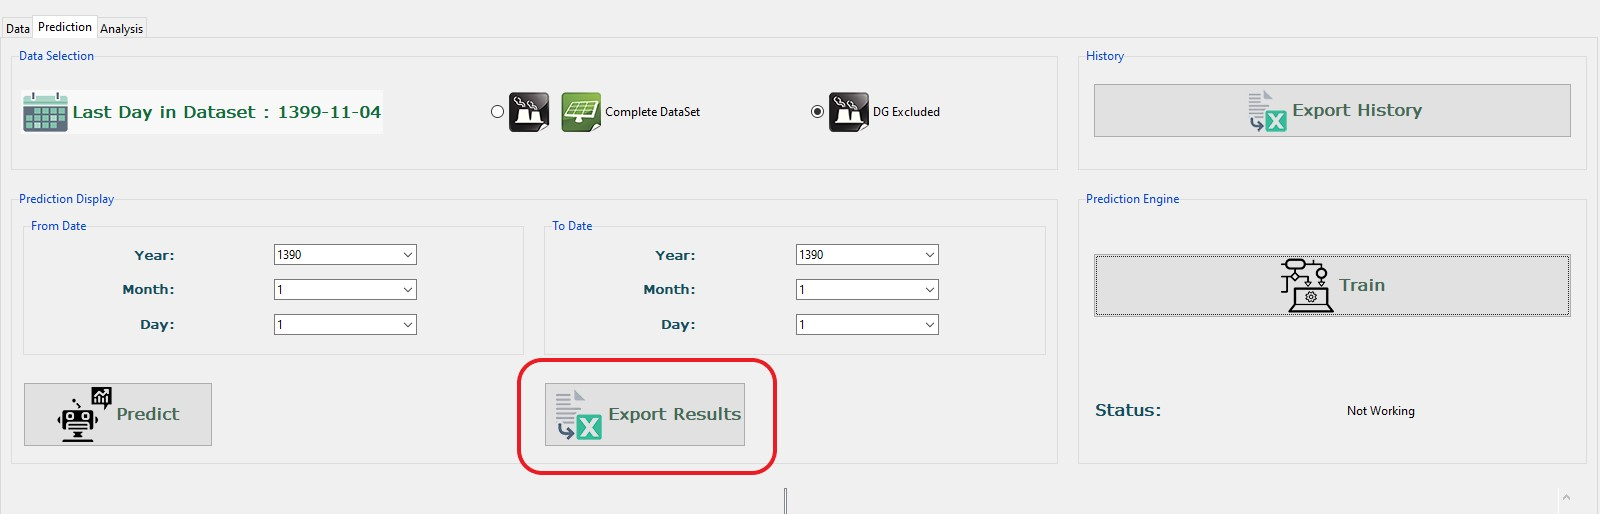
\includegraphics[width = \textwidth]{fig14}
	\caption{استخراج نتایج پیش‌بینی}
	\label{fig27}
\end{figure}
\section{دریافت تاریخچه پیش‌بینی‌ها}
برای دریافت تاریخچه پیش‌بینی‌هایی که توسط نرم‌افزار انجام شده در قالب اکسل، به زبانه
\lr{Prediction}
رفته و بر روی گزینه 
\lr{Export History}
کلیک کنید (شکل
\ref{fig40}
).

\begin{figure}[!h]
	\centering
	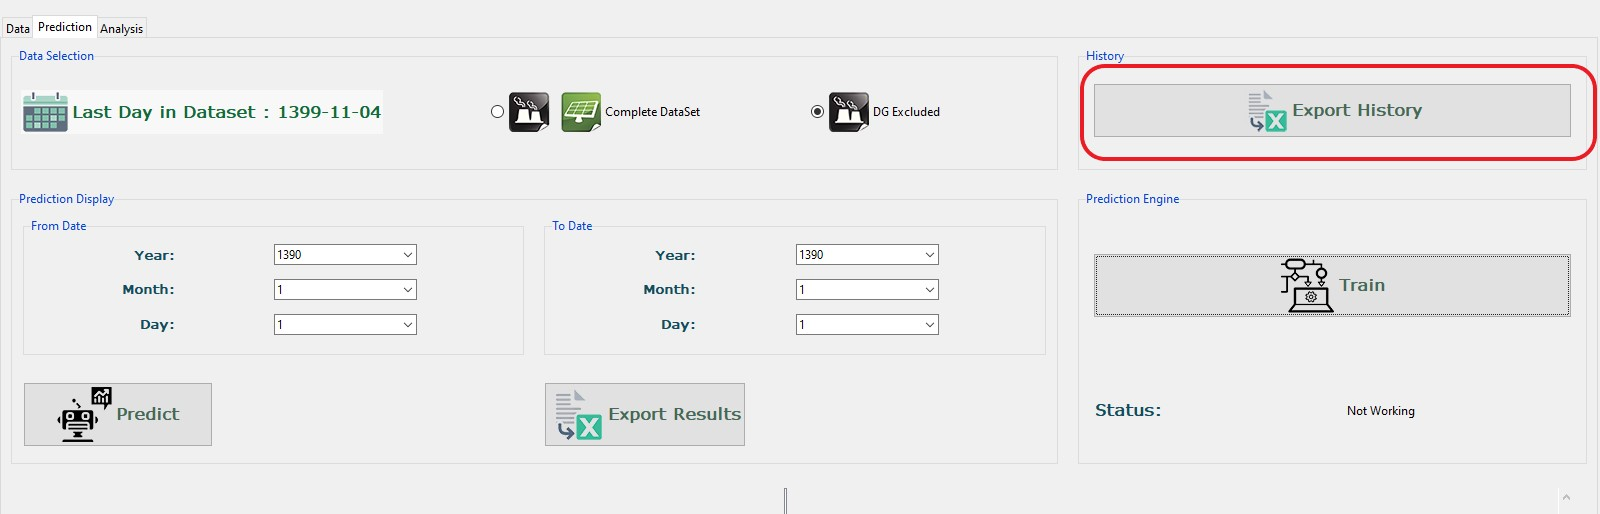
\includegraphics[width = \textwidth]{fig36}
	\caption{گرفتن تاریخچه پیش‌بینی‌ها}
	\label{fig40}
\end{figure}

اطلاعات مربوط به تمام پیش‌بینی‌هایی که انجام شده به همراه تاریخی که پیش‌بینی انجام شده است، در قالب یک فایل اکسل در محلی که انتخاب می‌کنید ذخیره خواهد شد.
\chapter{آنالیز پیش‌بینی}
در پهبار،‌امکان آنالیز پیش‌بینی‌های انجام شده توسط نرم‌افزار نیر وجود دارد. تمامی اطلاعات پیش‌بینی از ابتدای استفاده از نرم‌افزار در آن ذخیره شده است و می‌توانید به تجزیه و تحلیل آن‌ها بپردازید.

به این منظور، به زبانه
\lr{Analysis}
رفته و دیتاست مورد نظر را انتخاب کنید (شکل
\ref{fig34})

\begin{figure}[!h]
	\centering
	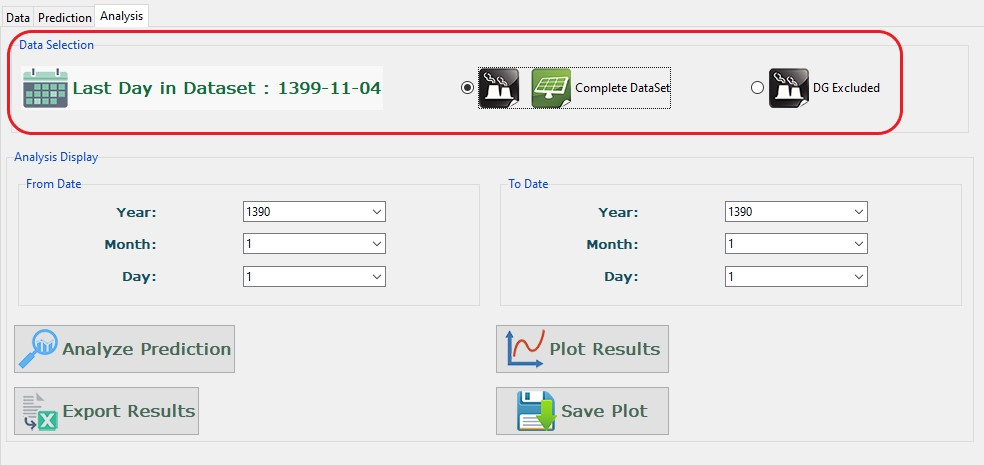
\includegraphics[width = \textwidth]{fig37}
	\caption{انتخاب دیتاست}
	\label{fig34}
\end{figure}
سپس بازه مورد نظر را انتخاب نمایید (شکل
\ref{fig32}).

\begin{figure}[!h]
	\centering
	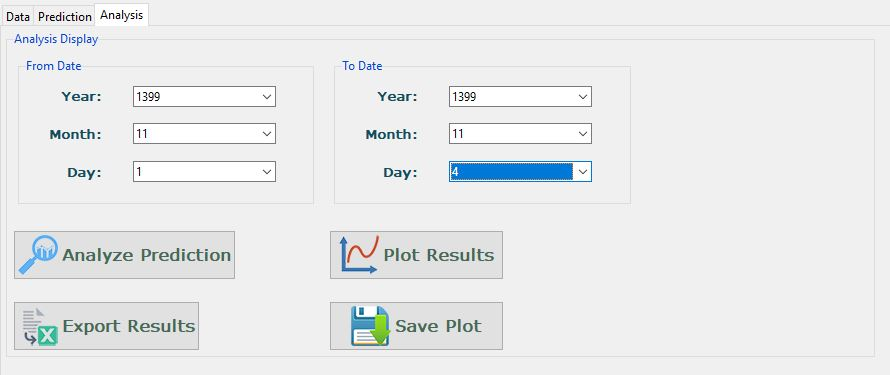
\includegraphics[width = \textwidth]{fig29}
	\caption{انتخاب بازه برای انجام آنالیز}
	\label{fig32}
\end{figure}
بر روی گزینه 
\lr{Analyze Prediction}
کلیک کنید.
در صورتی که بازه انتخاب شده در پیش‌بینی‌های انجام شده وجود نداشته باشد پیغام خطا نمایش داده خواهد شد.

در صورت وجود اطلاعات پیش‌بینی، آنالیز انجام شده و پیغام زیر به همراه نتایج، نمایش داده می‌شود (شکل
\ref{fig35}).

\begin{figure}[!h]
	\centering
	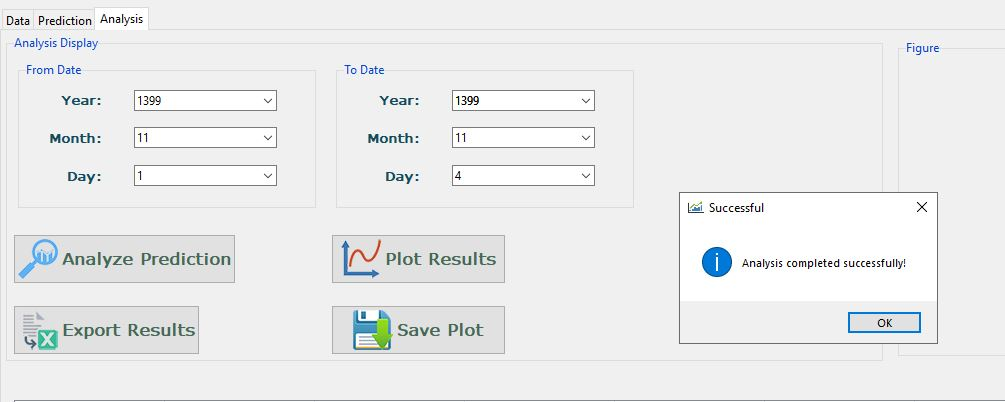
\includegraphics[width = \textwidth]{fig31}
	\caption{انجام موفقیت‌آمیز آنالیز خطا}
	\label{fig35}
\end{figure}

در صورت تمایل به استخراج نتایج، بر روی گزینه 
\lr{Export Results}
کلیک (
\ref{fig36}
) و فایل اکسل حاوی اطلاعات آنالیز را در یک فایل اکسل ذخیره نمایید.

\begin{figure}[!h]
	\centering
	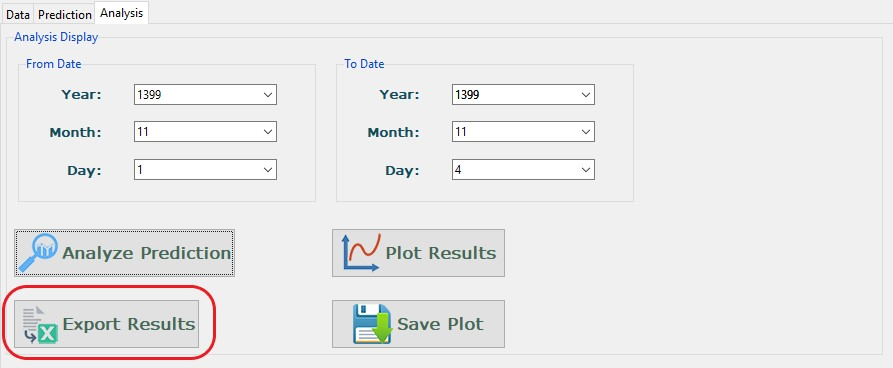
\includegraphics[width = \textwidth]{fig32}
	\caption{استخراج نتایج}
	\label{fig36}
\end{figure}
امکان رسم نمودارهای مقادیر واقعی و پیش‌بینی شده و هم‌چنین خطا نیز برای بازه‌هایی که آنالیز خطا انجام شده، ‌وجود دارد.

بدین منظور، پس از انجام آنالیز، روز مورد نظر برای رسم نمودار را از قسمت انتخاب بازه، انتخاب کنید و بر روی گزینه
\lr{Plot Results}
کلیک کنید (شکل
\ref{fig37}). 

\begin{figure}[!h]
	\centering
	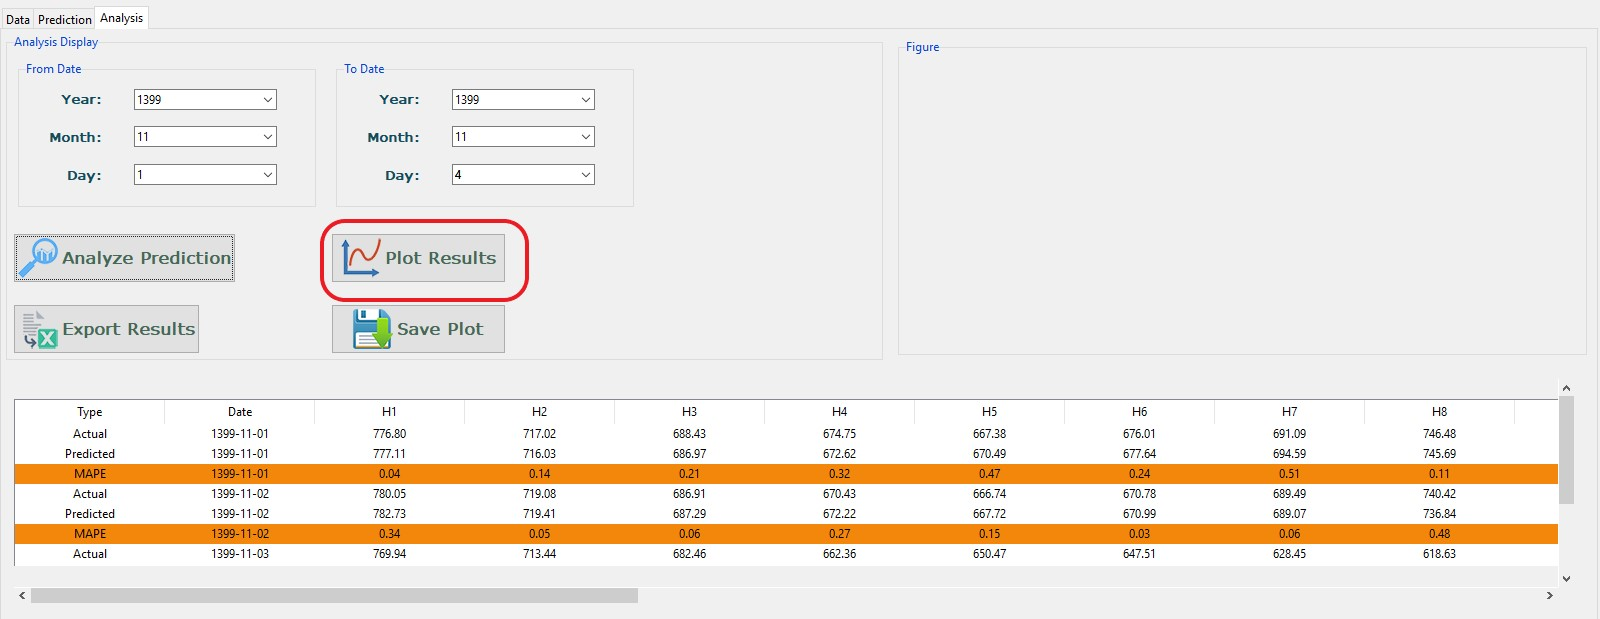
\includegraphics[width = \textwidth]{fig33}
	\caption{رسم نمودار آنالیز پیش‌بینی}
	\label{fig37}
\end{figure}

\textcolor{red}{نرم‌افزار پهبار،‌در حال حاضر فقط امکان نمایش نمودار مربوط به یک روز را دارد. بنابراین در قسمت انتخاب بازه، فقط یک روز را انتخاب نمایید. در غیر این صورت، پیغام خطا نمایش داده خواهد شد.}

نتایج رسم نمودارهای مربوط به یک روز موجود در اطلاعات آنالیز شده،‌ در شکل
\ref{fig38}
نشان داده شده است.

\begin{figure}[!h]
	\centering
	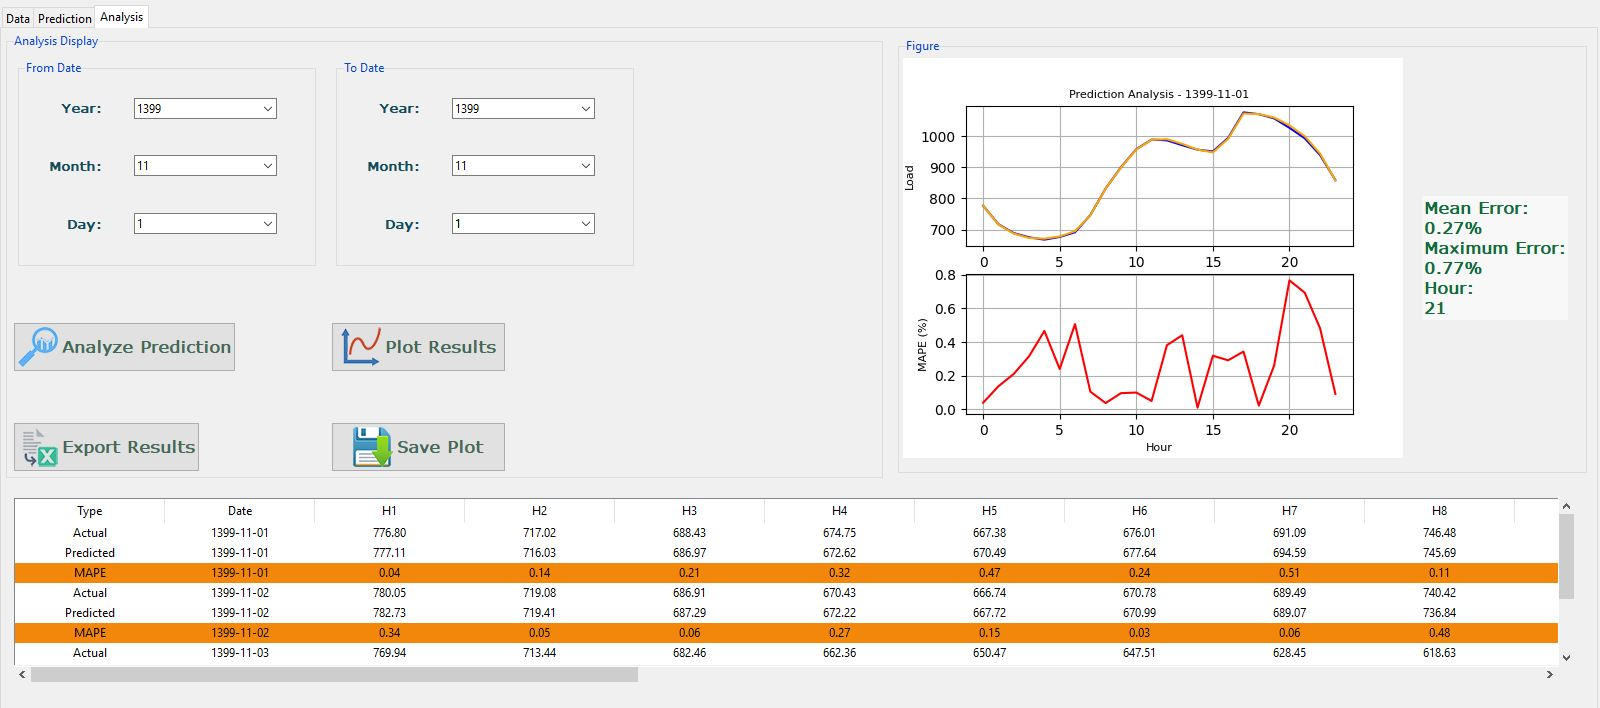
\includegraphics[width = \textwidth]{fig34}
	\caption{نتایج آنالیز و نمودارها}
	\label{fig38}
\end{figure}

با کلیک بر روی گزینه
\lr{Save Plot}
می‌توانید نمودار را در محل مورد نظر ذخیره کنید.
\end{document}
